\section{EMS - ED application}

\subsection{Application}

The system defined in section \ref{sec:model_overview} can be applied 
to a healthcare scenario with two such queueing systems.
The two queueing systems can be thought of as two Emergency Departments (ED) and 
the Emergency Medical Services (EMS) as a distributor that distributes 
patients to them.

There are numerous news articles that focus on the problems that arise when 
ambulances stay parked outside of the hospital for a long amount of time
~\cite{dailyrecords}, \cite{staffordshirelive}.
Some news reports also comment on the long idle time of ambulances when 
they are not in use~\cite{herefordtimes} and there are several reports of 
examples where this became an issue for new patients~\cite{southwalesargus}.
A particular article looked into this problem from the point of view of an 
ambulance paramedic:

\begin{quotation}
    % <!--alex ignore he-she her-him-->
    ``He knows if a patient arrives more urgently in need of help, his will be 
    pushed back''~\cite{bbcwales}

    ``We used to bring poorly patients in, and we were out on the road again in 15 minutes.''~\cite{bbcwales}
\end{quotation}

The patients that are distributed by the EMS arrive at the hospital via an 
ambulance and are then either unloaded at the ED or stay blocked outside in 
the ambulance.
Whether or not the ambulance and the patient stay blocked is determined by 
the threshold that the given ED chooses to play.
High threshold indicates that the ED accepts patients even if it is relatively 
full, while low threshold means that the ED blocks ambulances more frequently.

The parameters of the model correspond to the following parameters of the ED and 
the EMS:

\begin{itemize}
    \item \( \lambda_2 \): The rate of non-emergency patients that the EMS 
    receives
    \item \( \lambda_{1_i} \): The arrival rate of other patients to ED \(i\in\{1, 2\}\)
    \item \( \mu_i \): The service rate of patients at ED \(i\in\{1, 2\}\)
    \item \( C_i \): The number of available resources (beds) in ED \(i\in\{1, 2\}\)  
    \item \( T_i \): The action that ED \(i\in\{1, 2\} \) chooses to play which 
    corresponds to the threshold at which they do not accept EMS patients.
    \item \( N_i \): The total patient capacity of ED \(i\in\{1, 2\} \)
    \item \( M_i \): The total parking capacity of ED \(i\in\{1, 2\} \)
    \item \( R \): The time target for both EDs
    \item \( \alpha \in [0, 1] \) : \textit{Weighting} of blocking time and 
    lost individuals (equation \ref{eq:obj_distributor})
\end{itemize}

The strategies of the two EDs are the range of thresholds that they can choose
from and their utilities is the proportion of individuals whose time in the 
system is within a predetermined target time.
The EMS has to decide how to distribute its patients among the two EDs so that 
the weighted combination of the ambulance blocking time and the percentage of 
lost ambulances is minimised. 
As defined in \ref{sec:model_overview}, the interaction between the two EDs 
is a Normal form game that is then used to inform the decision of the EMS.
Note that the formulated game here assumes that prior to making a choice the 
EMS knows the strategies that each ED is playing (figure 
\ref{fig:imperfect_info_game}). This corresponds to reacting to experienced delays.

\subsection{Numerical Results}

This subsection aims to analyse how the gaming framework can affect the 
performance measures of the two hospitals and how to avoid certain inefficient 
situations.

The most commonly used method for analysing normal form games is the Nash 
equilibrium described in section \ref{sec:methodology_nash_equilibrium}
Consider the following game:

\begin{multicols}{3}
    \begin{itemize}
        \item \( \lambda_{1_1} \) = 1
        \item \( \mu_1 \) = 2
        \item \( C_1 \) = 2
        \item \( N_1 \) = 10
        \item \( M_1 \) = 6
        \columnbreak

        \item \( \lambda_{1_2} \) = 2
        \item \( \mu_2 \) = 2.5
        \item \( C_2 \) = 2
        \item \( N_2 \) = 10
        \item \( M_2 \) = 6
        \columnbreak

        \item \( \lambda_2 \) = 2
        \item \( R \) = 2
        \item \( \alpha \) = 0.5
    \end{itemize}
\end{multicols}

The set of possible actions to choose from for player 1 and player 2 is the
set of thresholds that the EDs can choose from: 
\begin{equation}
    T_1 = \{ 0, \ldots, N_1 \}, \quad T_2 = \{ 0, \ldots, N_2 \}
\end{equation}

For this example the only Nash equilibrium of the game is achieved when both 
players choose a threshold of \( T_1 = 10, T_2 = 10 \).
This means that the two players' best response to each other is to only block
ambulances when they are full. 

Nash equilibria is a theoretical measure which can be
inconsistent with intuitive notions about what should be the outcome of a 
game \cite{myerson1978refinements}.
Therefore it might not be the best way to describe human behaviour.
Since the work of Maynard Smith \cite{smith1986evolutionary} evolutionary game 
theory gives the tools for the emergence of stable behaviour.
One such model that allows for asymmetric payoffs, as is the case above, is 
replicator dynamics described in section 
(\ref{sec:methodology_learning_algorithms}).
Stable outcomes of this algorithm will correspond to a subset of Nash
equilibria but more importantly, will give a model of emergent behaviour. 

The use of a learning algorithm allows to investigate, not only the outcome of 
the game, but also how that outcome is reached.
Consider figure \ref{fig:ard_by_itself}. 
By running asymmetric replicator dynamics on the system the behaviour that 
emerges can be observed.
It can be seen that for this particular set of parameters the strategies of 
the two hospitals converge over time. 
Both hospital 1 (row player) and hospital 2 (column player) seem to be playing 
the same strategy \(s_{10}\) which indicates that thresholds \(T_1 = 10\) and 
\(T_2 = 10\) are played.
What is more important in this example is how the two hospitals reached these
decisions which also highlights the importance of using a learning algorithm.
Hospital 2 is able to reach the decision in a short amount of time while 
hospital 1 takes longer and goes through numerous strategies to get there.

\begin{figure}[H]
    \centering
    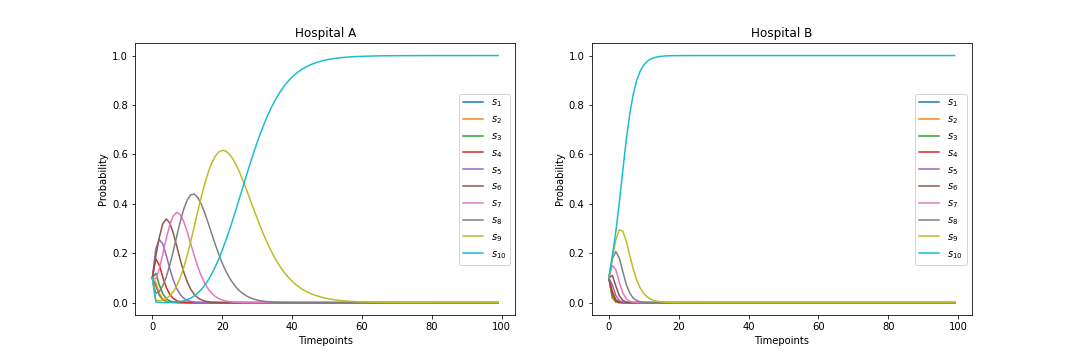
\includegraphics[scale=0.4, trim=120 0 120 0]{imgs/asymmetric_rd/asymmetric_rd.png}
    \caption{Asymmetric replicator dynamics run}
    \label{fig:ard_by_itself}
\end{figure}

In order to analyse how efficient the strategies played at every iteration are, 
the concept of the price of anarchy is used.
Price of anarchy is a measure that is used to quantify the efficiency of a
behaviour \cite{roughgarden2005selfish}.
In other words the price of anarchy is the worst-case equilibria measure and it 
is defined as:

\begin{equation}\label{eq:general_price_of_anarchy}
    \text{PoA} = \frac{\max_{s \in E} F(s)}{\min_{s \in S} F(s)}
\end{equation}

Here, \(S\) is the set of all sets of strategies \((s_1, s_2)\), \(E\) is the 
set of all possible sets of equilibria and \(F\) is the cost function to 
measure the efficiency for. 

To study the efficiency of the strategies being played a new concept is 
introduced that considers the ratio between each hospital's best achievable 
blocking time and the one that is being played.
This new concept is defined as the compartmentalised price of anarchy of the 
players of the game and is defined as \(PoA_i(\tilde{s})\), where 
\(i \in \{1, 2\}\) to distinguish among the two players/hospitals where 
\(\tilde{s}\) is the strategy that is being played by player \( i \). 
The compartmentalised price of anarchy aims to measure inefficiencies in the 
model.
The \(PoA\) for the blocking time of player \(i\) for strategy \(\tilde{s}\) 
is given by:

\begin{equation}\label{eq:poa_compartmentalised}
    PoA_{i}(\tilde{s}) = \frac{B_i(\tilde{s})}{\min_{s \in S_i} B_i(s)}
\end{equation}

Consider a game with two smaller (lower \( N_i, M_i \)) and busier (higher 
\(\lambda_{1_i} \) and \(\lambda_2\)) hospitals with the following set of 
parameters:

\begin{multicols}{3}
    \begin{itemize}        
        \item \( \lambda_{1_1} \) = 4.5
        \item \( \mu_1 \) = 2
        \item \( C_1 \) = 3
        \item \( T_1 \in [1, N_1] \) 
        \item \( N_1 \) = 6
        \item \( M_1 \) = 5

        \columnbreak
        \item \( \lambda_{1_2} \) = 6
        \item \( \mu_2 \) = 3
        \item \( C_2 \) = 2
        \item \( T_2 \in [1, N_2] \)
        \item \( N_2 \) = 7
        \item \( M_2 \) = 4
        
        \columnbreak
        \item \( \lambda_2 \) = 10.7
        \item \( R \) = 2
        \item \( \alpha \) = 0.9
    \end{itemize}
\end{multicols}

\textbf{Initial scenario:}
Using equation (\ref{eq:poa_compartmentalised}) and asymmetric replicator 
dynamics the emergent behaviour can be measured and the compartmentalised price 
of anarchy at every iteration for both players.
Figure \ref{fig:ard_original} shows the strategies that are being played and 
the values of \(PoA_1(s)\) and \(PoA_2(s)\) for all iterations of the 
learning algorithm until it reaches an evolutionary stable pair of strategies.

\begin{figure}[H]
    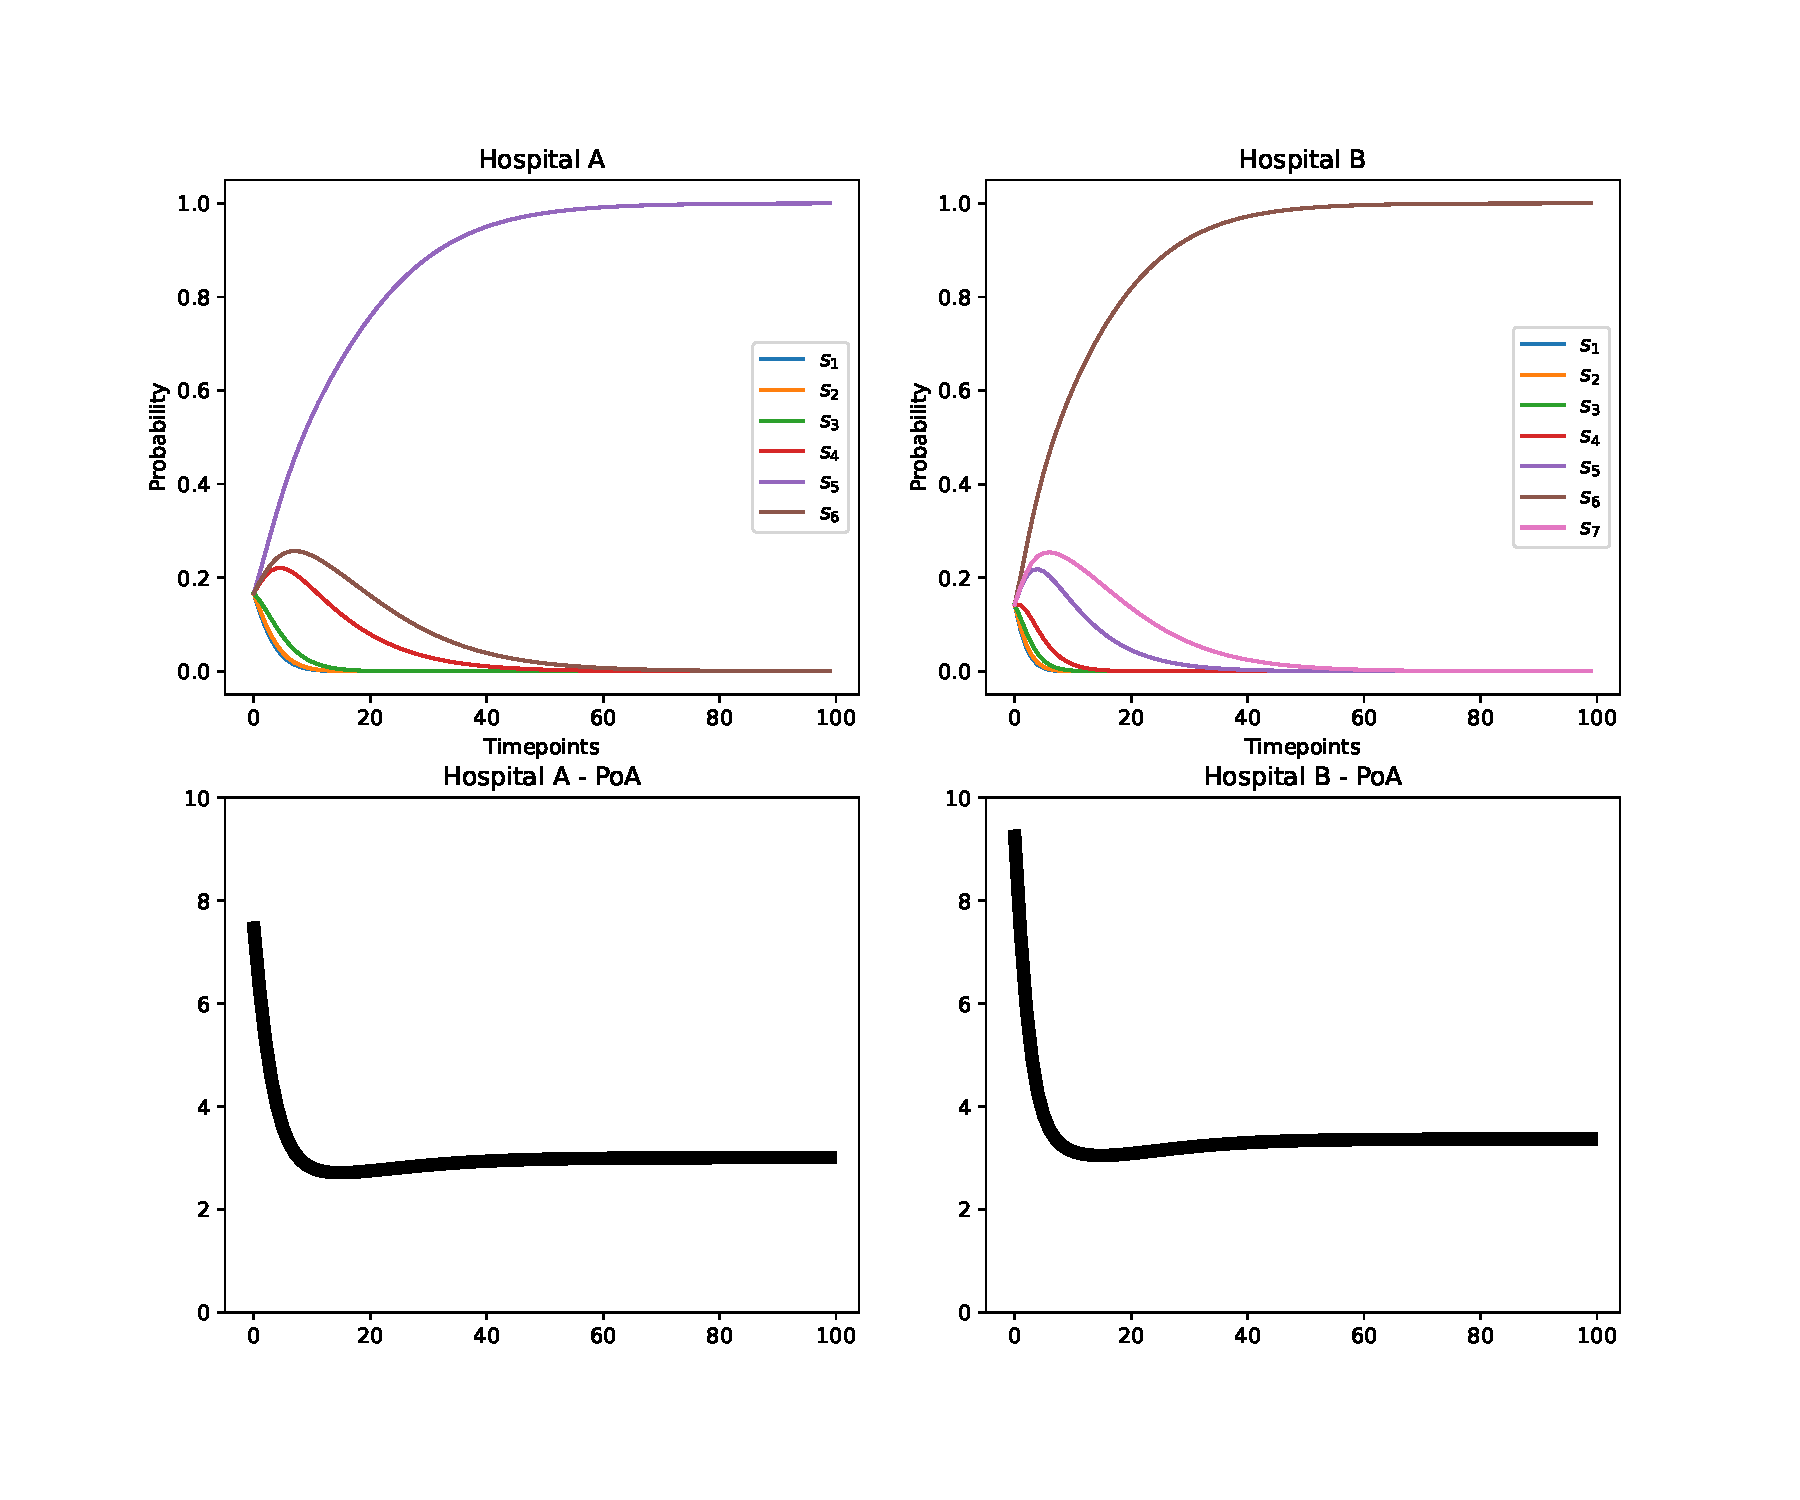
\includegraphics[width=\textwidth]{imgs/asymmetric_rd_and_PoA/asymmetric_original.pdf}
    \caption{The strategies played when running asymmetric replicator dynamics
    along with the compartmentalised price of anarchy of the blocking time at
    each iteration of the learning algorithm}
    \label{fig:ard_original}
\end{figure}

The learning algorithm reaches a stable pair of 
strategies where \(T_1 = 5\) and \(T_2 = 6\). After a number of iterations the
price of anarchy for both players stabilises and barely increases until the 
final iteration. 

\textbf{Increasing \(\lambda_2\):}
Figure \ref{fig:ard_lambda_2} shows a similar run of the
algorithm but when the strategies begin to stabilise an increase in the
arrival rate of ambulances occurs (i.e \( \lambda_2 = 24 \)).


\begin{figure}[H]
    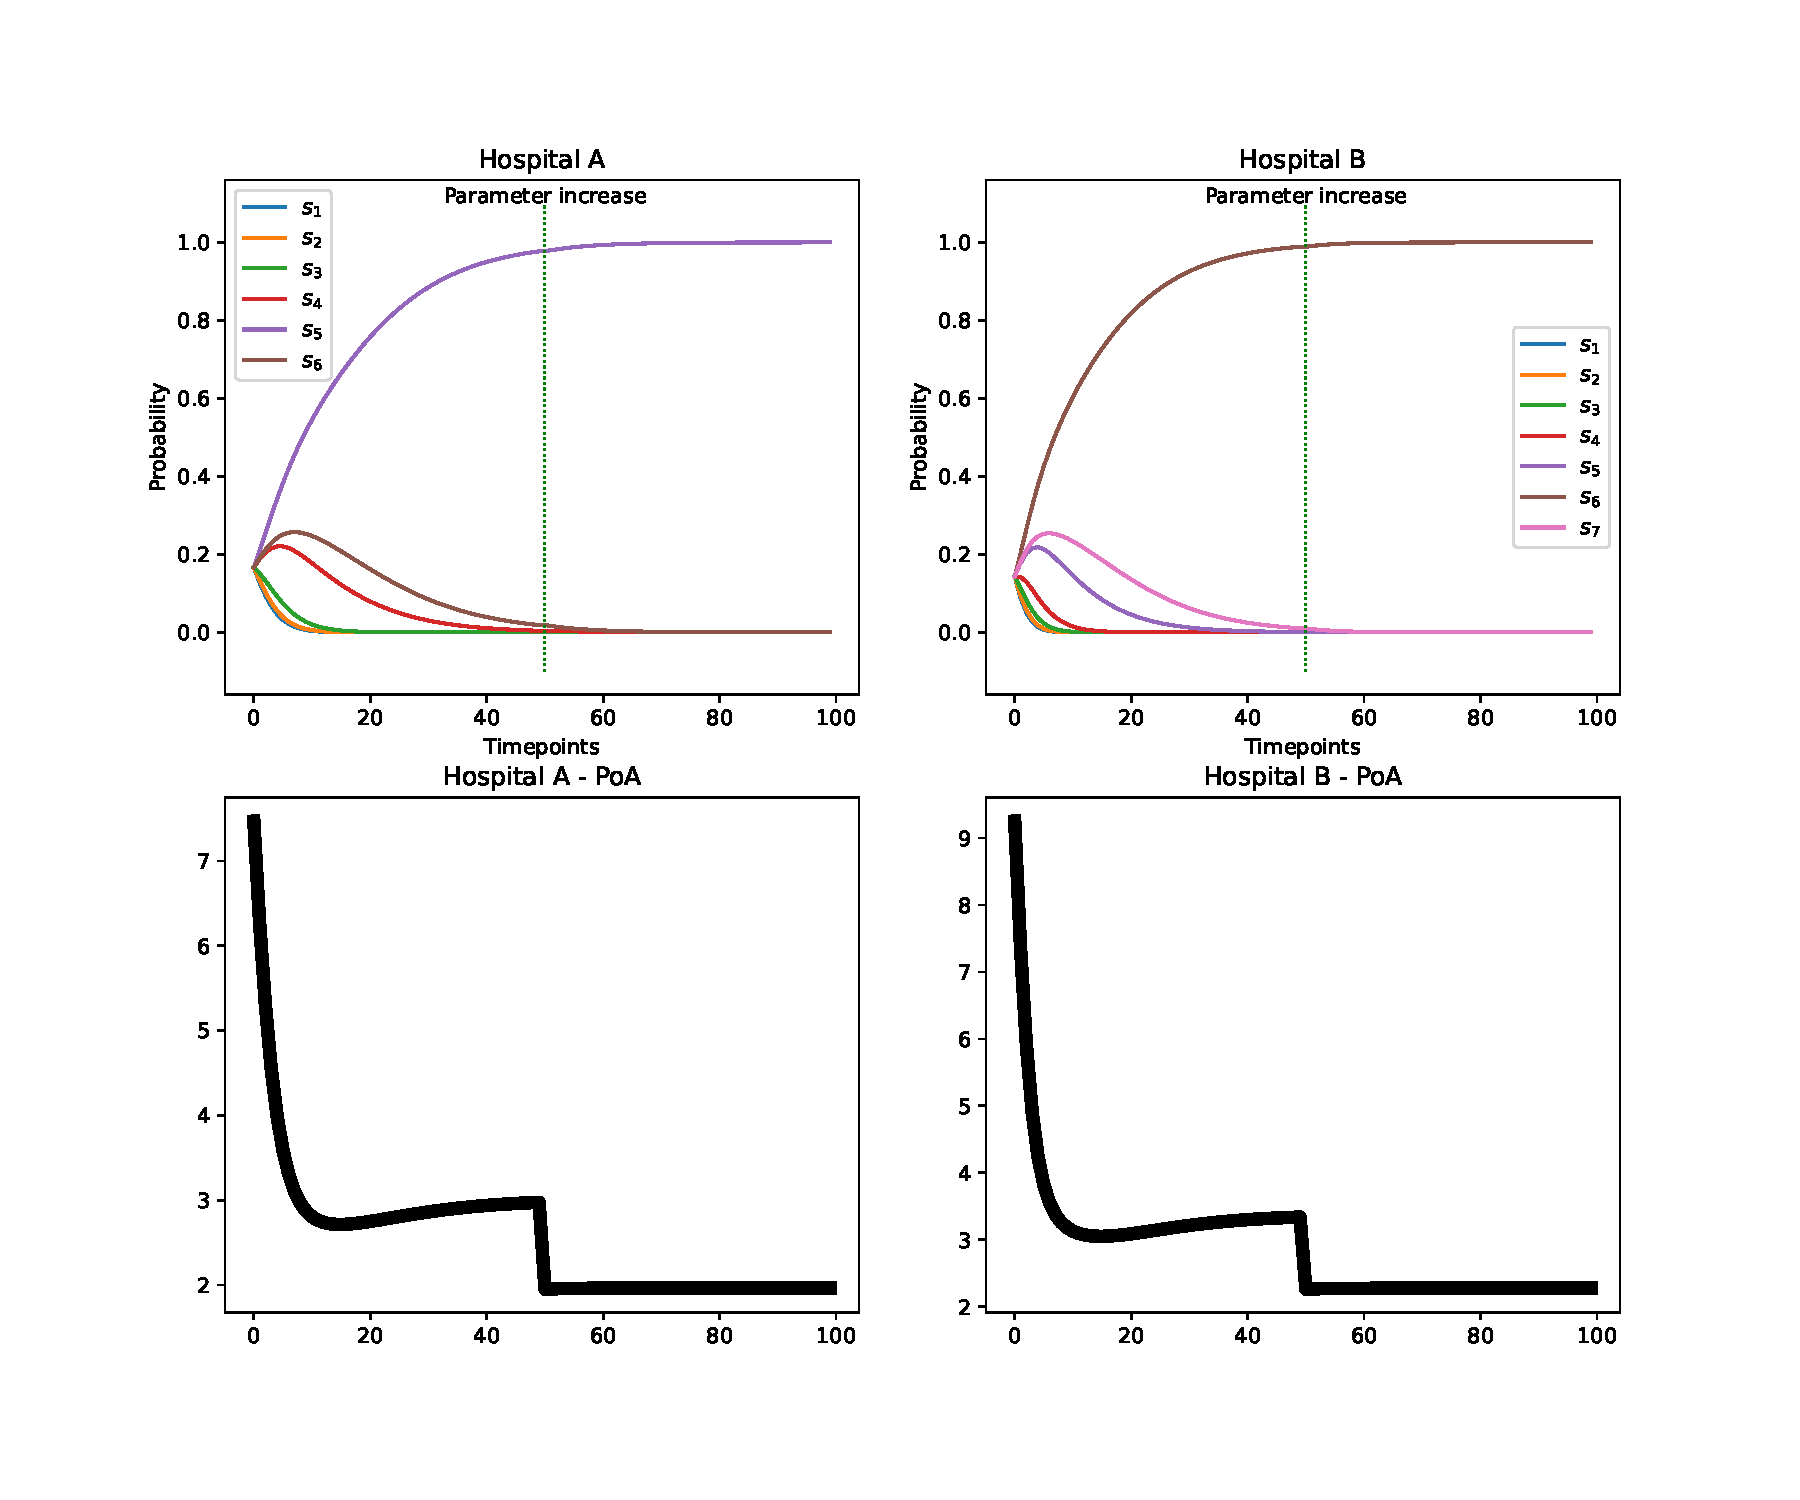
\includegraphics[width=\textwidth]{imgs/asymmetric_rd_and_PoA/asymmetric_flooding.pdf}
    \caption{The strategies played when running asymmetric replicator dynamics
    along with the compartmentalised price of anarchy of the blocking time at
    each iteration of the learning algorithm. After a number of iterations the 
    arrival rate of ambulance patients is significantly increased to flood the
    system completely \( \lambda_2 = 24 \).}
    \label{fig:ard_lambda_2}
\end{figure}


By increasing \(\lambda_2\) there is no change as to how players behave
(\(T_1 = 5, T_2 = 6\)), but the efficiency of the system does change. 
There is a decline in the price of anarchy of the blocking time which at first 
glance indicates that upon flooding the system it becomes the loss in efficiency
due to rational individual behaviour decreases. 
This is non-sensical though.
What it really shows is that the steep increase in \( \lambda_2 \) leaves 
the system unable to cope regardless of the decisions made.

\textbf{Increasing number of servers \( C_1 \) and \( C_2 \):}
Figure \ref{fig:ard_num_of_servers} shows a run of asymmetric replicator 
dynamics with a change in the number of servers of the hospitals.
The number of servers are increased from \(C_1 = 3, C_2 = 2\) to 
\(C_1 = 4, C_2 = 3\).


\begin{figure}[H]
    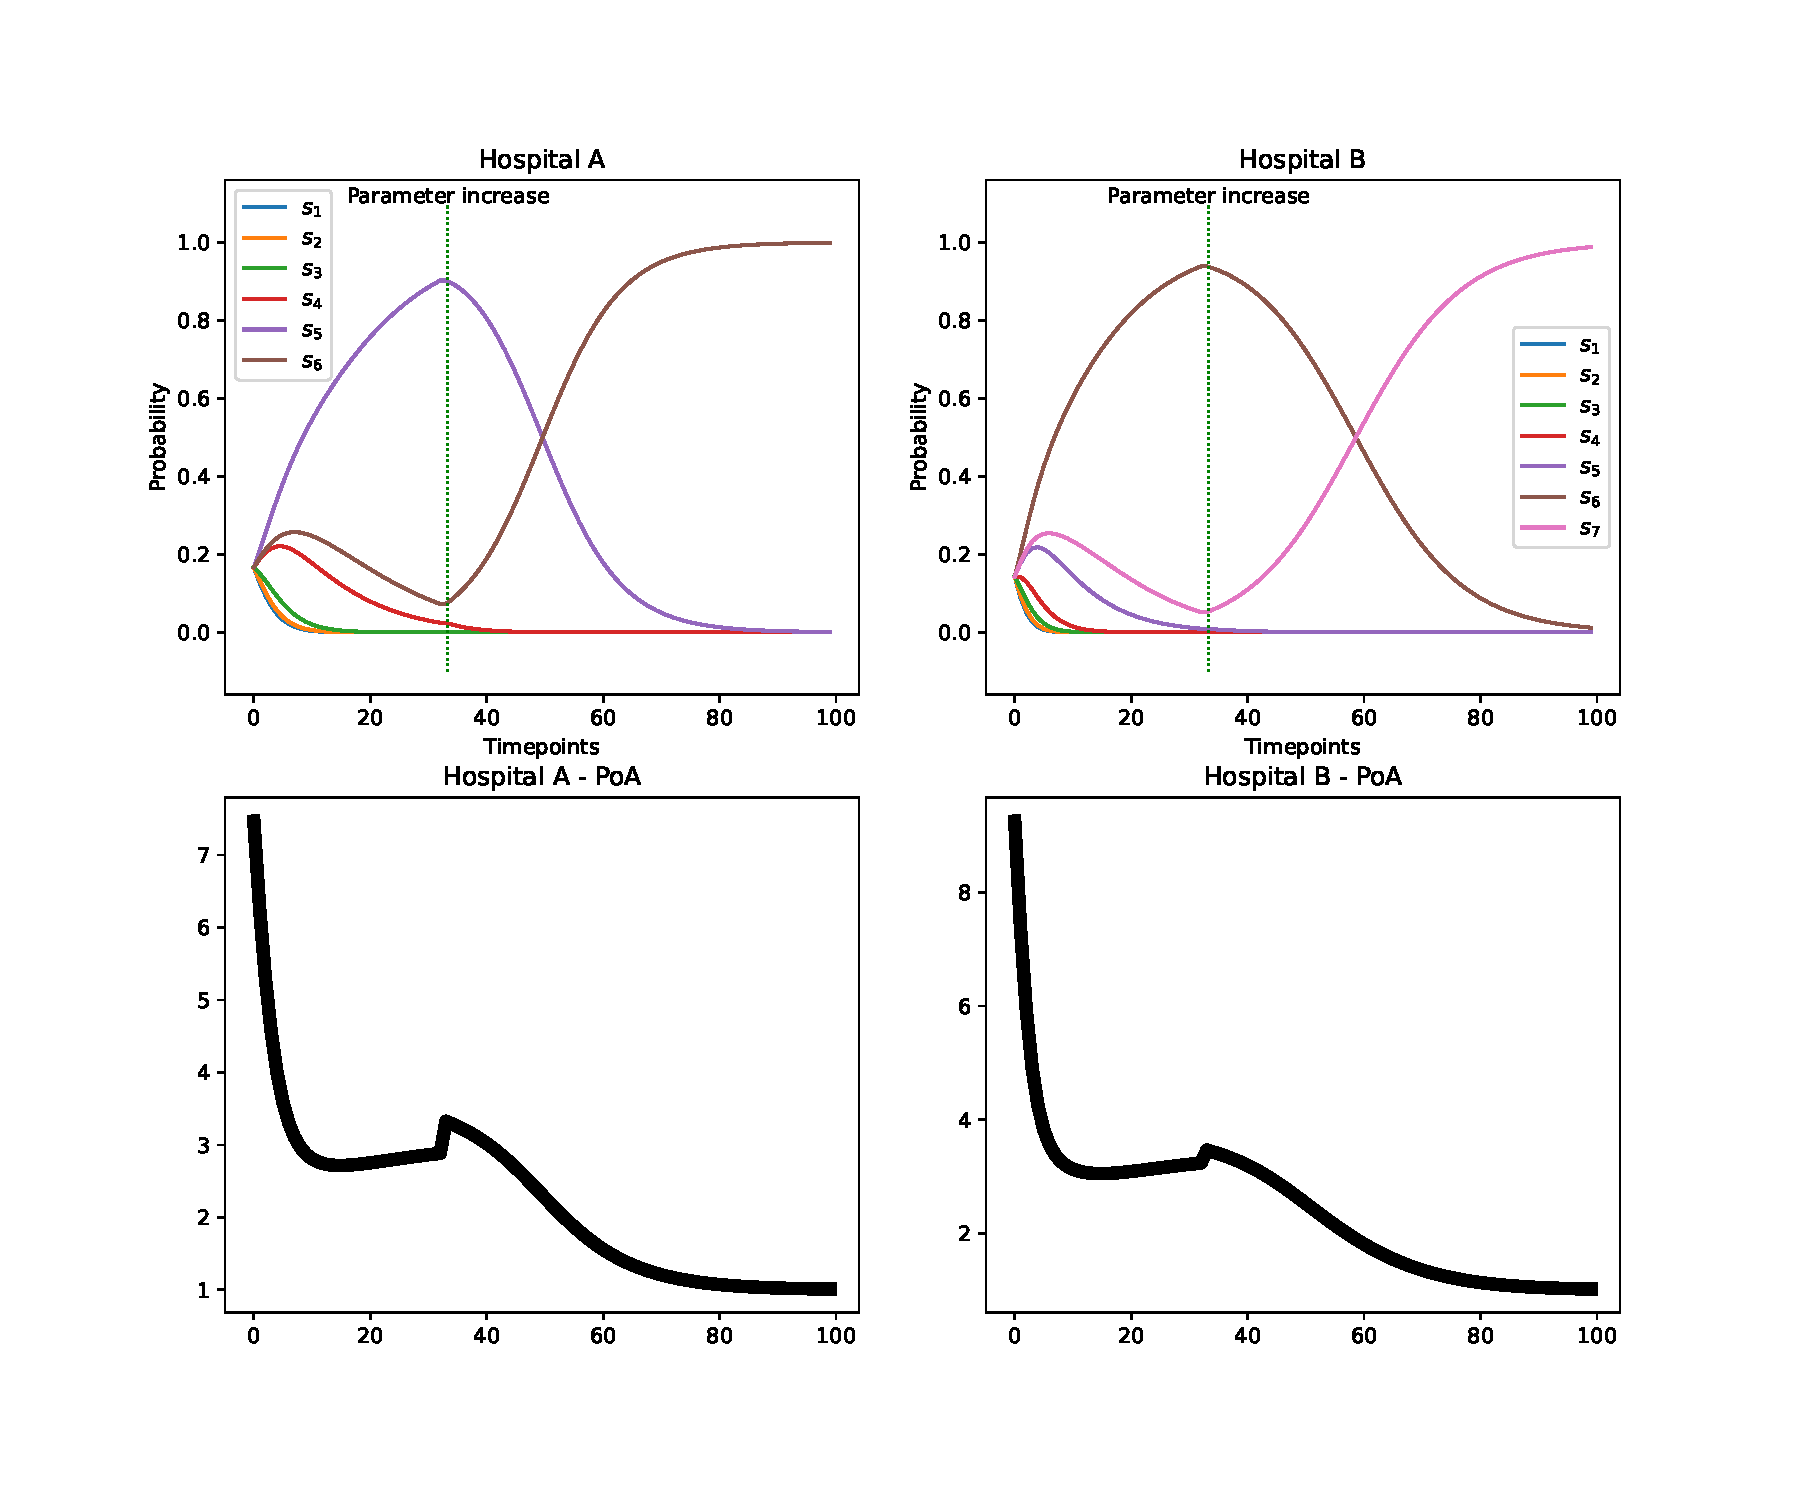
\includegraphics[width=\textwidth]{imgs/asymmetric_rd_and_PoA/asymmetric_increase_C.pdf}
    \caption{
        The strategies played when running asymmetric replicator dynamics
        along with the compartmentalised price of anarchy of the blocking time 
        at each iteration of the learning algorithm. After a number of 
        iterations the number of servers for both systems are increased by one.
    }
    \label{fig:ard_num_of_servers}
\end{figure}

In this case, both the behaviour as well as the price of anarchy change.
The players change their strategies from \(T_1 = 5, T_2 = 6\) to 
\(T_1 = 6, T_2 = 7\) and the \(PoA\) of the blocking time goes down.
By adding more resources to the models they are able to increase their 
efficiency.
Although this is a good way to escape such inefficiencies, it might not always
be cost efficient.

\textbf{Incentivising players:}
From figures \ref{fig:ard_lambda_2} and \ref{fig:ard_num_of_servers} it can be
seen that we can change some parameters of the model to make it more efficient.
The approach used on figure \ref{fig:ard_penalty} is slightly different than 
the previous cases.
Once the played strategies in asymmetric replicator dynamics strategies 
converge the payoff matrices of the two are scaled in such a way so that the 
utilities of the selected strategy are penalised. This corresponds to a precise
policy change where more societally beneficial behaviours are incentivised.

Matrices \(A\) and \(B\) represent the original payoff matrices while matrices
\(\tilde{A}\) and \(\tilde{B}\) represent the incentivised payoff matrices.
It can be observed that matrix \(\tilde{A}\) is a scaled version of matrix 
\(A\) only on the row that is most frequently played and similarly matrix 
\(\tilde{B}\) of matrix \(B\) only on the column that is most frequently played
(matrix \(A\): row \(5\), matrix \(B\): column \(6\), see figure 
\ref{fig:ard_penalty}).
Note that the values of the payoff matrices only differ on the fourth digit
which is the raw utility of the strategies played.

\tiny
\begin{equation*}
    A = 
    \begin{bmatrix}
        0.9995052 & 0.9995052 & 0.9995052 & 0.9995052 & 0.9995052 
        & 0.9995052 & 0.9995052 \\
        0.99954989 & 0.99954978 & 0.99954961 & 0.99954924 & 0.99954845 
        & 0.9995466 & 0.999539 \\
        0.99968233 & 0.99968194 & 0.99968151 & 0.99968067 & 0.99967874 
        & 0.9996734 & 0.999649  \\
        0.99990299 & 0.99990245 & 0.99990189 & 0.99990081 & 0.99989832
        & 0.9998909 & 0.9998517 \\
        \color{blue}0.99999996 & \color{blue}0.99999994 & \color{blue}0.99999992 
        & \color{blue}0.99999988 & \color{blue}0.99999973 & \color{blue}0.9999989 
        & \color{blue}0.9999859 \\
        0.9998773 & 0.99987995 & 0.99988236 & 0.99988643 & 0.99989417 
        & 0.9999126 & 0.9999712
    \end{bmatrix}
\end{equation*}

\begin{equation*}
    B = 
    \begin{bmatrix}
        0.99917127 & 0.99925823 & 0.99946188 & 0.99968499 & 0.9998942 
        & \color{red}1.0 & 0.99982128 \\
        0.99917127 & 0.99925479 & 0.99945638 & 0.99968051 & 0.99989153 
        & \color{red}0.99999997 & 0.9998333  \\
        0.99917127 & 0.99924532 & 0.99943793 & 0.99966451 & 0.99988286 
        & \color{red}0.99999966 & 0.99985269 \\
        0.99917127 & 0.99924146 & 0.99942878 & 0.99965484 & 0.99987667 
        & \color{red}0.99999921 & 0.99986701 \\
        0.99917127 & 0.9992342 &  0.99941013 & 0.99963286 & 0.99986077 
        & \color{red}0.9999972 & 0.9998958  \\
        0.99917127 & 0.99921279 & 0.99934961 & 0.99954933 & 0.99978407 
        & \color{red}0.99997106 & 0.99997276 \\
    \end{bmatrix}
\end{equation*}

\begin{equation*}
    \tilde{A} = 
    \begin{bmatrix}
        0.99950518 & 0.99950518 & 0.99950518 & 0.99950518 & 0.99950518
        & 0.99950518 & 0.99950518 \\
        0.99954989 & 0.99954978 & 0.99954961 & 0.99954924 & 0.99954845
        & 0.99954656 & 0.99953879 \\
        0.99968233 & 0.99968194 & 0.99968151 & 0.99968067 & 0.99967874
        & 0.99967339 & 0.9996492  \\
        0.99990299 & 0.99990245 & 0.99990189 & 0.99990081 & 0.99989832
        & 0.9998909 & 0.99985171 \\
        \color{blue}0.99969996 & \color{blue}0.99969994 & \color{blue}0.99969992 
        & \color{blue}0.99969988 & \color{blue}0.99969973 & \color{blue}0.99969895 
        & \color{blue}0.99968586 \\
        0.9998773 &  0.99987995 & 0.99988236 & 0.99988643 & 0.99989417
        & 0.99991264 & 0.99997122 \\
    \end{bmatrix}
\end{equation*}

\begin{equation*}
    \tilde{B} = 
    \begin{bmatrix}
        0.99917127 & 0.99925823 & 0.99946188 & 0.99968499 & 0.9998942
        & \color{red}0.9997 & 0.99982128 \\
        0.99917127 & 0.99925479 & 0.99945638 & 0.99968051 & 0.99989153
        & \color{red}0.99969997 & 0.9998333 \\
        0.99917127 & 0.99924532 & 0.99943793 & 0.99966451 & 0.99988286
        & \color{red}0.99969966 & 0.99985269 \\
        0.99917127 & 0.99924146 & 0.99942878 & 0.99965484 & 0.99987667
        & \color{red}0.99969921 & 0.99986701 \\
        0.99917127 & 0.9992342 &  0.99941013 & 0.99963286 & 0.99986077
        & \color{red}0.9996972 & 0.9998958 \\
        0.99917127 & 0.99921279 & 0.99934961 & 0.99954933 & 0.99978407
        & \color{red}0.99967106 & 0.99997276 \\
    \end{bmatrix}
\end{equation*}
\normalsize


\begin{figure}[H]
    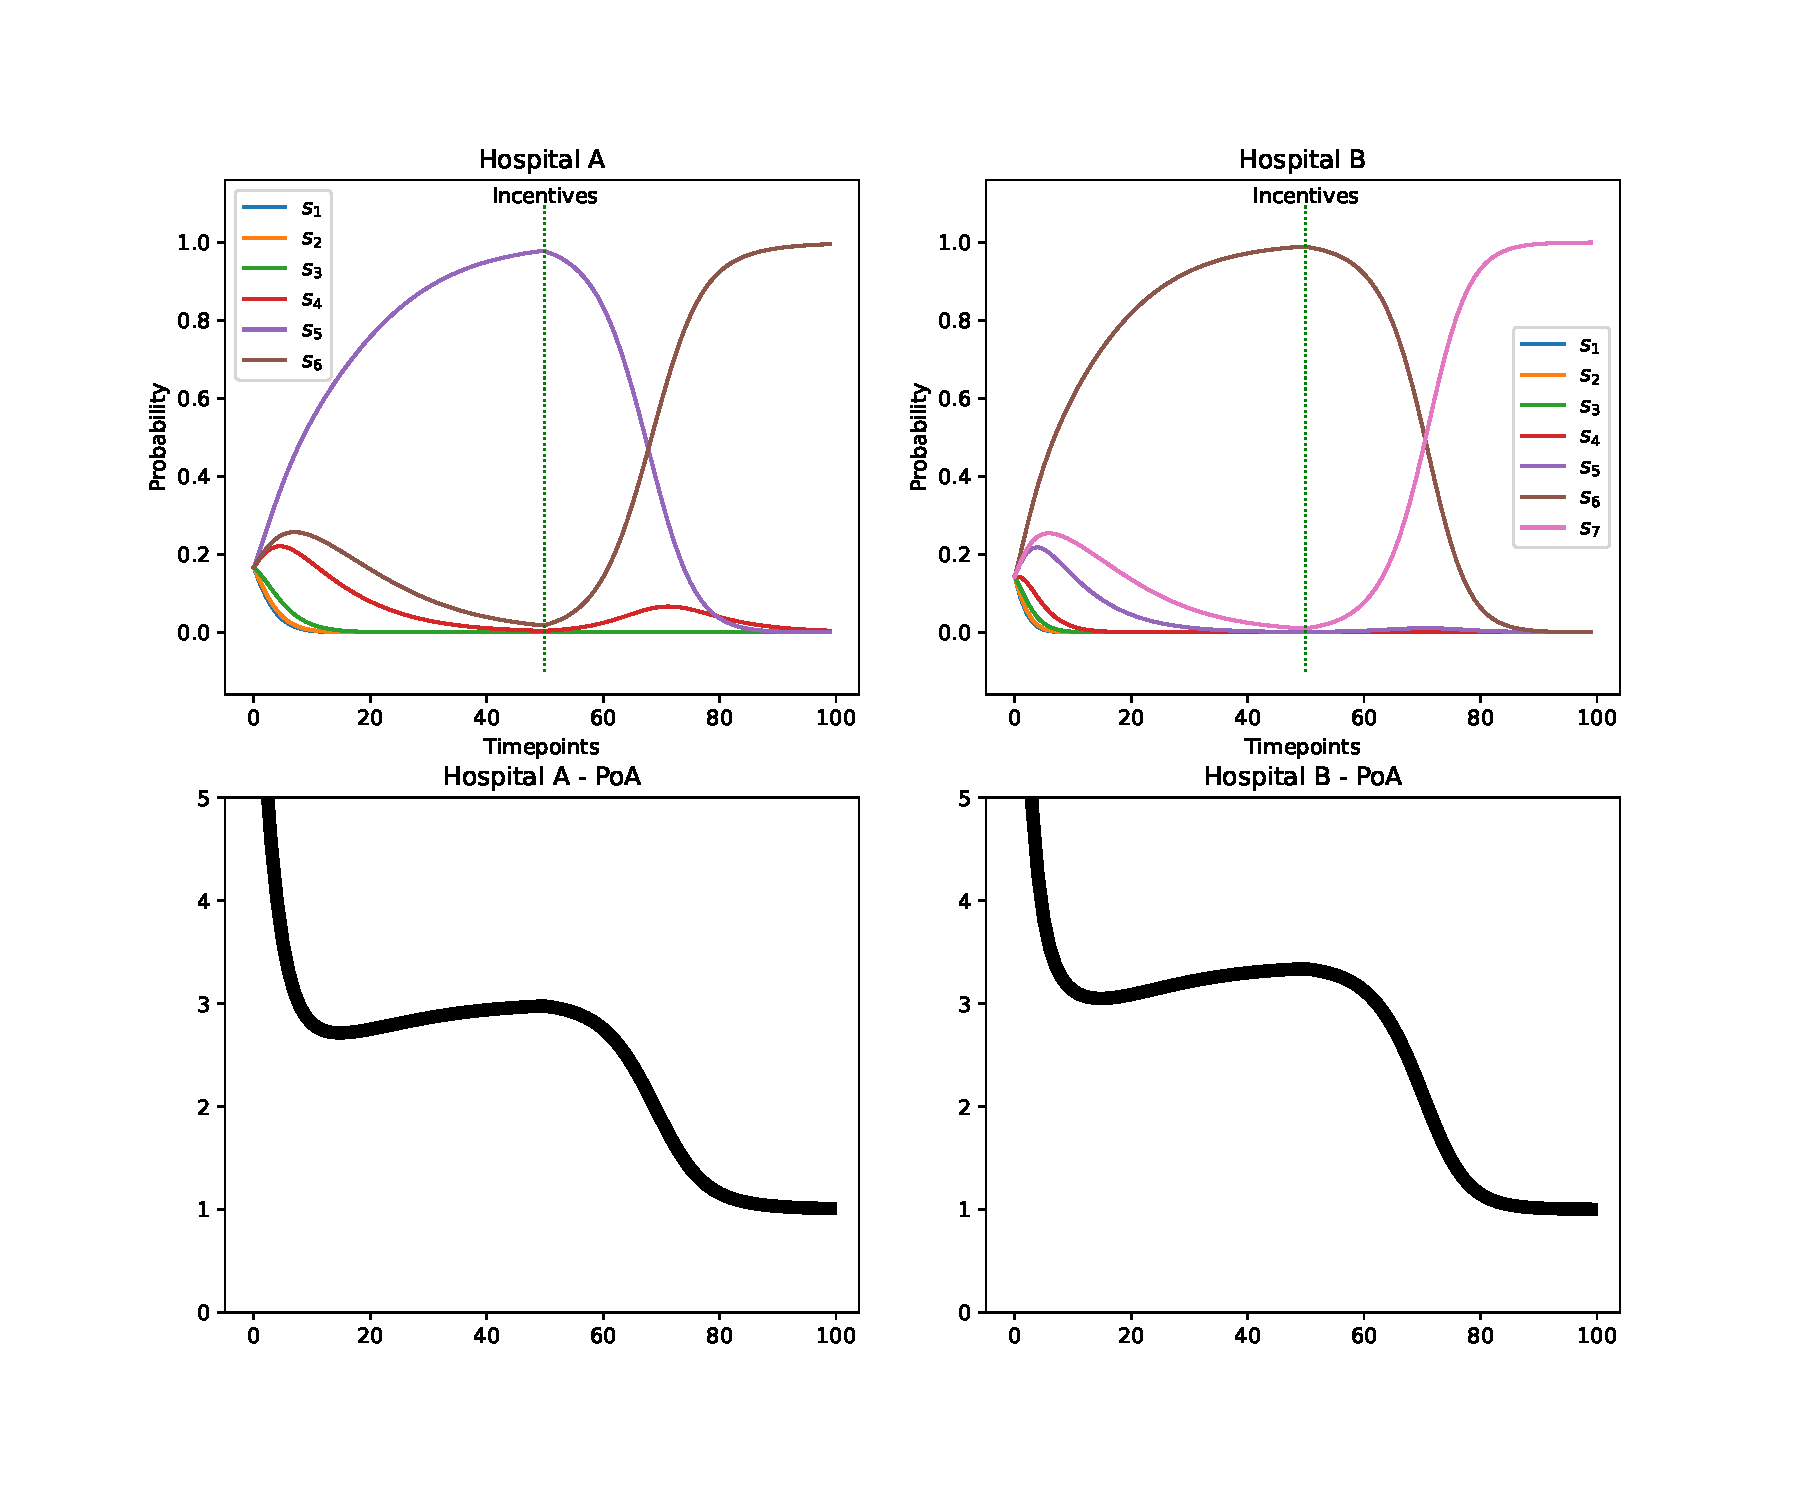
\includegraphics[width=\textwidth]{imgs/asymmetric_rd_and_PoA/asymmetric_penalty.pdf}
    \caption{
        The strategies played when running asymmetric replicator dynamics
        along with the compartmentalised price of anarchy of the blocking time 
        at each iteration of the learning algorithm. After a number of 
        iterations the most dominant strategy is being penalised.
    }
    \label{fig:ard_penalty}
\end{figure}

Figure \ref{fig:ard_penalty} shows that players start playing strategies 
\( T_1 = 5\) and \( T_2 = 6 \) and mid-run of the learning algorithm a penalty
is applied to these strategies on the payoff matrix.
By incentivising the players in such a way the players change their strategies 
to \(T_1 = 6\) and \(T_2 = 7\), and thus ambulance patients are accepted in the 
ED more often.
Hence, the \(PoA\) for both EDs is decreased, meaning that the whole system is
more efficient in terms of the blocking time.
